\documentclass[11pt]{article}
%Gummi|065|=)
\usepackage[title]{appendix}
\usepackage{hyperref}
\usepackage{amsmath}
\usepackage{graphicx}
\title{\textbf{Jensen's Inequality}}
\author{K{\i}van\c{c} \c{C}akmak\\}
\date{}
\begin{document}

\maketitle

This blog post aims to prove the Jensen's inequality, which states that for a random variable $x$ and a concave function $f(x)$ , the following equation holds: 

\begin{equation}
E[f(x)] \leq f(E[f(x)]) 
\end{equation}

i.e.

\begin{equation}
\sum_{i=1}^k p_{i} f(x_{i}) \leq f(\sum_{i=1}^k p_{i} f(x_{i})) 
\end{equation}

\section{Preliminary Definitions on Concave and Convex}

A function of a single variable is concave, if every line segment joining two points on its graph does not lie above the graph at any point. Symmetrically, a function of a single variable is convex if every line segment joining two points on its graph does not lie below the graph at any point - See Figure \ref{fig:concave_convex_neither}. \\

\begin{figure} \label{fig:concave_convex_neither}
\centering
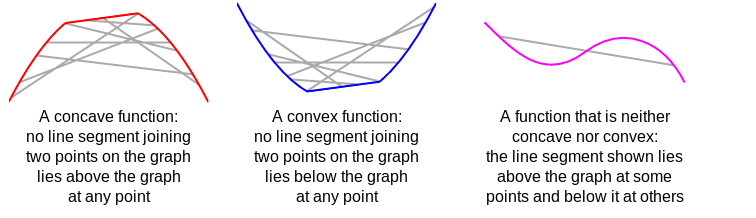
\includegraphics[width=\textwidth]{img/concave_convex_neither.png}
\caption{concave, convex, neither}
\end{figure}

\begin{figure} \label{fig:concave}
\centering
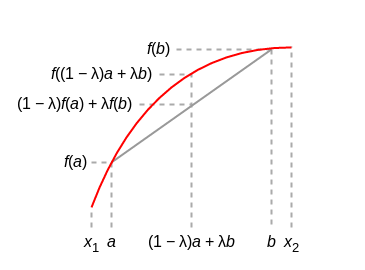
\includegraphics[width=0.7\textwidth]{img/concave.png}
\caption{concave function}
\end{figure}

\begin{equation}
f((1-\lambda)a + \lambda b) \geq (1-\lambda)f(a) + \lambda f(b), \textit{  concave}
\end{equation}

\begin{equation}
f((1-\lambda)a + \lambda b) \leq (1-\lambda)f(a) + \lambda f(b), \textit{  convex}
\end{equation}

\section{Proof}

Suppose f is differentiable. The function f is concave if, for any x and y:

\begin{equation}
f(x) \leq f(y) + (x-y) f^{\prime}(y)
\end{equation}

Let $x = X$ and $y = E[X]$. \\

We can write: 

\begin{equation}
f(X) \leq f(E[X]) + (X - E[X])f^{\prime}(E[X]) 
\end{equation}

This inequality is true for all X , so we can take expectation on both sides to get

\begin{equation}
E[f(x)] \leq f(E[X]) + f^{\prime}(E[X])E[(X - E[X])] = f(E[X]) 
\end{equation}

since we can say that 

\begin{equation}
E[X] = \mu \\
\end{equation}
\begin{equation}
E[(X - E[x])] = E[X - \mu] = E[X] - E[\mu] = \mu - \mu = 0 
\end{equation}

\begin{thebibliography}{99}


\bibitem{a1}
\url{https://mjo.osborne.economics.utoronto.ca/index.php/tutorial/index/1/cv1/t}

\bibitem{a2}
\url{http://www.sef.hku.hk/~wsuen/teaching/micro/jensen.pdf }
\end{thebibliography}

\end{document}
